\documentclass[10pt,aspectratio=169]{beamer}
\usepackage[english]{babel}
\usepackage{lmodern,amsmath,amssymb,mathtools,array,booktabs,graphicx,tikz}
\usetikzlibrary{arrows.meta,positioning,calc,fit}
\makeatletter\def\input@path{{theme/}}\makeatother
\providecommand{\draftmode}{0}
\usetheme{inria}
\graphicspath{{assets/}}
\setbeamercolor{normal text}{fg=inria-noir,bg=white}
\setbeamercolor{alerted text}{fg=inria-rouge}
\setbeamertemplate{navigation symbols}{}
\hypersetup{pdftitle={Multi-Modal, Training-Free Crack Extraction via Generalized Frangi Graph},
 pdfauthor={Louis Hauseux; Raphaël Antoine; Philippe Foucher; Pierre Charbonnier; Josiane Zerubia},
 pdfsubject={EUVIP 2026 oral presentation, paper 81, 29 September 2026},
 colorlinks=true,urlcolor=inria-2024-bleu-canard,linkcolor=inria-noir}
\newcommand{\Frangi}{{\rmfamily\mdseries\textsc{Frangi}}}
\newcommand{\Hess}{\mathcal H}
% Shared bibliographic records for inline citations, page notes and bibliography.
\makeatletter
\newcommand{\DeclareRef}[4]{%
 \expandafter\gdef\csname ref@label@#1\endcsname{#2}%
 \expandafter\gdef\csname ref@authors@#1\endcsname{#3}%
 \expandafter\gdef\csname ref@details@#1\endcsname{#4}}
\newcommand{\DeclareShort}[2]{%
 \expandafter\gdef\csname ref@short@#1\endcsname{#2}}
\newcommand{\DeclareMyRef}[4]{%
 \DeclareRef{#1}{#2}{#3}{#4}%
 \expandafter\gdef\csname ref@mine@#1\endcsname{}}
\newcommand{\refcheck}[1]{%
 \ifcsname ref@label@#1\endcsname\else
  \PackageError{euvip-citations}{Unknown reference #1}{Declare it in references.tex.}%
 \fi}
\newcommand{\refcolor}[1]{%
 \ifcsname ref@mine@#1\endcsname\color{inria-rouge}%
 \else\color{gris_fonce_inria}\fi}
\newcommand{\refbracket}[1]{%
 \refcheck{#1}{\refcolor{#1}\bfseries[\csname ref@label@#1\endcsname]}}
\newcommand{\citb}[1]{\mbox{{\scriptsize\refbracket{#1}}}}
\newcommand{\reffoot}[1]{%
 \begin{textblock}{.90}[0,1](.05,.917)
  \begingroup
  \fontsize{5.5}{6.4}\selectfont\raggedright
  \setlength{\parindent}{0pt}\setlength{\parskip}{0pt}%
  \edef\rf@list{\zap@space#1 \@empty}%
  \@for\rf@key:=\rf@list\do{%
   \refcheck{\rf@key}%
   {\refcolor{\rf@key}%
    \noindent\refbracket{\rf@key}\space
    \ifcsname ref@short@\rf@key\endcsname
     \csname ref@short@\rf@key\endcsname
    \else
     \csname ref@authors@\rf@key\endcsname\space
     \csname ref@details@\rf@key\endcsname
    \fi\par}}%
  \endgroup
 \end{textblock}}
\newcommand{\bibentry}[1]{%
 \refcheck{#1}\par\vspace{2.3mm}%
 \begin{minipage}[t]{.23\linewidth}\footnotesize\refbracket{#1}\end{minipage}\hfill
 \begin{minipage}[t]{.75\linewidth}\raggedright\refcolor{#1}%
  {\footnotesize\csname ref@authors@#1\endcsname\par}%
  {\scriptsize\csname ref@details@#1\endcsname\par}%
 \end{minipage}\par}
\makeatother

\DeclareRef{frangi98}{Frangi 98}
 {A.~F.~Frangi, W.~J.~Niessen, K.~L.~Vincken, M.~A.~Viergever.}
 {``Multiscale vessel enhancement filtering.'' MICCAI,~1998.}
\DeclareMyRef{gretsi25}{GRETSI 25}
 {L.~Hauseux, R.~Antoine, P.~Foucher, P.~Charbonnier, J.~Zerubia.}
 {``Généralisation du filtre de Frangi pour l'extraction des réseaux de fissures au sein d'images d'un glissement de terrain. Comparaison avec une méthode d'apprentissage profond.'' GRETSI,~2025.}
\DeclareMyRef{euvip26}{EUVIP 26}
 {L.~Hauseux, R.~Antoine, P.~Foucher, P.~Charbonnier, J.~Zerubia.}
 {``Multi-Modal, Training-Free Crack Extraction via Generalized Frangi Graph.'' EUVIP,~2026.}
\DeclareRef{find22}{FIND 22}
 {S.~Zhou, C.~Canchila, W.~Song.}
 {``Fused Image dataset for convolutional neural Network-based crack Detection (FIND).'' Zenodo,~2022. \href{https://zenodo.org/records/6383044}{Dataset record}.}
\DeclareRef{cracksegdiff24}{CrackSegDiff 24}
 {X.~Jiang, L.~Jiang, A.~Wang, K.~Zhu, Y.~Gao.}
 {``CrackSegDiff: Diffusion Probability Model-based Multi-modal Crack Segmentation.'' \href{https://arxiv.org/abs/2410.08100}{arXiv:2410.08100}, 2024.}
\DeclareMyRef{ans26}{ANS 26}
 {L.~Hauseux, K.~Avrachenkov, J.~Zerubia.}
 {``Generalization of Single-Linkage with higher-order interactions.'' Applied Network Science, 11, article~9, 2026.}
\DeclareRef{sam23}{SAM 23}
 {A.~Kirillov et al.}
 {``Segment Anything.'' ICCV, pp.~4015--4026, 2023. \href{https://openaccess.thecvf.com/content/ICCV2023/html/Kirillov_Segment_Anything_ICCV_2023_paper.html}{Paper}.}
\DeclareRef{cracksam24}{CrackSAM 24}
 {K.~Ge, C.~Wang, Y.~Guo, Y.~Tang, Z.~Hu, H.~Chen.}
 {``Fine-tuning vision foundation model for crack segmentation in civil infrastructures.'' Construction and Building Materials, 431, 136573, 2024. \href{https://doi.org/10.1016/j.conbuildmat.2024.136573}{DOI}.}

% One-line page notes. The bibliography slides keep the complete records above.
\DeclareShort{frangi98}
 {A.~F.~Frangi et al., ``Multiscale vessel enhancement filtering.'' MICCAI,~1998.}
\DeclareShort{gretsi25}
 {L.~Hauseux et al., ``Généralisation du filtre de Frangi pour l'extraction des réseaux de fissures\ldots'' GRETSI,~2025.}
\DeclareShort{euvip26}
 {L.~Hauseux et al., ``Multi-Modal, Training-Free Crack Extraction via Generalized Frangi Graph.'' EUVIP,~2026.}
\DeclareShort{find22}
 {S.~Zhou et al., ``Fused Image dataset for convolutional neural Network-based crack Detection (FIND).'' Zenodo,~2022.}
\DeclareShort{cracksegdiff24}
 {X.~Jiang et al., ``CrackSegDiff: Diffusion Probability Model-based Multi-modal Crack Segmentation.'' arXiv,~2024.}
\DeclareShort{ans26}
 {L.~Hauseux, K.~Avrachenkov, J.~Zerubia. ``Generalization of Single-Linkage with higher-order interactions.'' Appl.~Netw.~Sci.,~2026.}
\DeclareShort{sam23}
 {A.~Kirillov et al., ``Segment Anything.'' ICCV,~2023.}
\DeclareShort{cracksam24}
 {K.~Ge et al., ``Fine-tuning vision foundation model for crack segmentation in civil infrastructures.'' Constr.~Build.~Mater.,~2024.}

\newcommand{\panel}[3]{\begin{minipage}[t]{#1\linewidth}\centering
 \includegraphics[width=\linewidth]{#2}\par\vspace{.8mm}{\scriptsize #3\par}\end{minipage}}
\newcommand{\divider}[2]{\section{#2}\begin{frame}[plain,noframenumbering]
 \vfill\centering{\Huge\bfseries #1\par}\vspace{3mm}
 {\LARGE\bfseries #2\par}\vspace{3mm}\barrecouleur\vfill\end{frame}}
\makeatletter
\setbeamertemplate{footline}{\leavevmode\hspace*{\hmargin}%
 \raisebox{.4\footerheight}{\parbox{\dimexpr\paperwidth-2\hmargin}{%
 \fontsize{5.7}{6.5}\selectfont EUVIP 2026\enspace |\enspace 29 September 2026\hfill
 \smash{\raisebox{-.1\footerheight}{\footerlogo}}\kern1.8em
 \makebox[2.2em][r]{\ifbeamer@noframenumbering\else\insertframenumber/10\fi}}}}
\makeatother
\date{29 September 2026}
\title{Multi-Modal, Training-Free Crack Extraction\\via Generalized Frangi Graph}
\author{Louis Hauseux et al.}

\begin{document}

\begin{frame}[plain,noframenumbering]
\begin{tikzpicture}[remember picture,overlay]
 \node[anchor=north west,inner sep=0] at ([xshift=.05\paperwidth,yshift=-.07\paperheight]current page.north west){\titlelogo};
 \node[anchor=north east,fill=white,inner xsep=3mm,inner ysep=2mm]
  at ([xshift=-.05\paperwidth,yshift=-.07\paperheight]current page.north east)
  {
\includegraphics[width=2.7cm]{cerema-official.pdf}};
 \node[anchor=north west,align=left,text width=.895\paperwidth,inner sep=0]
 at ([xshift=.055\paperwidth,yshift=-.285\paperheight]current page.north west){%
  {\fontsize{18}{21}\selectfont\bfseries Multi-Modal, Training-Free Crack Extraction\\via Generalized \Frangi{} Graph}\par
  \vspace{2mm}\barrecouleur\par\vspace{4mm}
  {\large European Workshop on Visual Information Processing\enspace --\enspace Luxembourg}\par\vspace{1mm}
  {\small 29 September 2026\enspace |\enspace Paper 81}\par\vspace{5mm}
  {\small Louis {\rmfamily\textsc{Hauseux}}\textsuperscript{1}, Raphaël {\rmfamily\textsc{Antoine}}\textsuperscript{2},
  Philippe {\rmfamily\textsc{Foucher}}\textsuperscript{2}, Pierre {\rmfamily\textsc{Charbonnier}}\textsuperscript{2},
  Josiane {\rmfamily\textsc{Zerubia}}\textsuperscript{1}}\par\vspace{3mm}
  {\footnotesize\textsuperscript{1}Inria, Université Côte d'Azur, Ayana research team, France\\
  \textsuperscript{2}Cerema, ENDSUM research team, France}\par\vspace{2mm}
  {\footnotesize\href{mailto:louis.hauseux@inria.fr}{louis.hauseux@inria.fr}}};
\end{tikzpicture}
\end{frame}

\begin{frame}[t]{Problem setting}
\vspace{1mm}
\begin{columns}[T,onlytextwidth]
 \begin{column}{.53\textwidth}
  \panel{.48}{Intensity_1FIND.png}{Intensity \citb{find22}}\hfill
  \panel{.48}{Range_1FIND.png}{Range / depth \citb{find22}}
 \end{column}
 \begin{column}{.43\textwidth}
  \begin{itemize}\setlength\itemsep{5mm}
   \item Cracks are \textbf{thin}, \textbf{weak} and often \textbf{discontinuous}.
   \item Several modalities may observe the same geometry.
   \item Goal: an \textbf{editable crack skeleton}, \textbf{without training} \citb{euvip26}
  \end{itemize}
 \end{column}
\end{columns}
\reffoot{find22,euvip26}
\end{frame}

\divider{01}{From pixels to a \Frangi{} graph}

\begin{frame}[t]{Classical \Frangi{} filter}
\vspace{-1mm}
\[
 \Hess_\sigma(x)=\nabla^2(G_\sigma*I)(x), \qquad |\lambda_1|\le |\lambda_2|.
\]
\vspace{-1mm}
\begin{columns}[c,onlytextwidth]
\begin{column}{.42\textwidth}\centering
\resizebox{.86\linewidth}{!}{%
\begin{tikzpicture}[x=1cm,y=1cm,
 ridge/.style={line width=9pt,gris_fonce_inria!55,line cap=round},
 vec/.style={-{Latex[length=2.4mm]},line width=1.1pt}]
 \begin{scope}[rotate=27]
  \draw[ridge](-2.05,0)--(2.05,0);
  \draw[inria-rouge,line width=1pt,fill=inria-rouge!8](0,0)ellipse(1.75 and .62);
  \draw[vec,inria-rouge](0,0)--(1.833,0);
  \draw[vec,inria-rouge!62](0,0)--(0,.703);
  \node[font=\small,inria-rouge,fill=white,inner sep=1pt]at(.95,0){$e_1$};
  \node[font=\small,inria-rouge!62,fill=white,inner sep=1pt]at(-.36,.40){$e_2$};
 \end{scope}
 \fill[inria-2024-bleu-canard](0,0)circle(2.1pt);
 \node[below left,font=\small]at(0,0){$x$};
\end{tikzpicture}}
\par\vspace{1.5mm}{\scriptsize Local ridge geometry \citb{frangi98}}
\end{column}
\begin{column}{.54\textwidth}
\begin{itemize}\setlength\itemsep{4mm}
 \item \textbf{Shape}: $R_B=|\lambda_1|/|\lambda_2|$
 \item \textbf{Contrast}: $S=\sqrt{\lambda_1^2+\lambda_2^2}$
\end{itemize}
\vspace{3mm}
\[
F_\sigma(x)=\exp\!\left(-\frac{R_B^2}{2\beta^2}\right)
\left(1-\exp\!\left(-\frac{S^2}{2c^2}\right)\right)
\]
\end{column}
\end{columns}
\reffoot{frangi98}
\end{frame}

\begin{frame}[t]{Generalized \Frangi{} graph}
\vspace{1mm}
\begin{columns}[c,onlytextwidth]
\begin{column}{.56\textwidth}\centering
\resizebox{\linewidth}{!}{%
\begin{tikzpicture}[x=1cm,y=1cm,
 ridge/.style={line width=7pt,gris_fonce_inria!45,line cap=round},
 dir/.style={-{Latex[length=1.9mm]},line width=1pt},
 pix/.style={circle,fill=inria-2024-bleu-canard,inner sep=0pt,minimum size=3.8pt}]
 \draw[ridge](-.15,-.3)--(2.75,.62);
 \node[pix](i1)at(.72,-.02){};\node[pix](j1)at(1.88,.35){};
 \draw[dir,inria-rouge](i1)--++(.62,.2);\draw[dir,inria-rouge](j1)--++(.62,.2);
 \draw[inria-rouge,line width=1.6pt](i1)--(j1);
 \node[font=\footnotesize,align=center]at(1.3,1.45){aligned axes\\strong edge};
 \begin{scope}[shift={(4.35,0)}]
  \draw[ridge](-.15,-.3)--(2,.4);\draw[ridge](1.3,.92)--(2.32,-.48);
  \node[pix](i2)at(.72,-.02){};\node[pix](j2)at(1.66,.43){};
  \draw[dir,inria-rouge](i2)--++(.59,.19);\draw[dir,inria-rouge](j2)--++(.36,-.5);
  \draw[gris_fonce_inria!45,line width=.8pt](i2)--(j2);
  \node[font=\footnotesize,align=center]at(1.2,1.45){misaligned axes\\weak edge};
 \end{scope}
\end{tikzpicture}}
\par\vspace{2mm}{\scriptsize Pairwise orientation alignment \citb{gretsi25}\enspace\citb{euvip26}}
\end{column}
\begin{column}{.40\textwidth}
\begin{itemize}\setlength\itemsep{4mm}
 \item Pixels become \textbf{nodes}.
 \item Ridge compatibility becomes \textbf{edge similarity}.
 \item \textcolor{inria-rouge}{\textbf{Alignment}} refines intensity and shape information.
\end{itemize}
\vspace{2mm}
\[
S^{(0)}_{ij}=\max_{\sigma\in\Sigma} 
S^\sigma_{\mathrm{int}}S^\sigma_{\mathrm{shape}}S^\sigma_{\mathrm{align}}
\]
\end{column}
\end{columns}
\reffoot{gretsi25,euvip26}
\end{frame}

\begin{frame}[t]{Multimodal fusion}
\vspace{1mm}
\begin{columns}[T,onlytextwidth]
\begin{column}{.52\textwidth}
\begin{enumerate}\setlength\itemsep{4mm}
 \item Normalize each Hessian
 \[
 \widehat\Hess_\sigma^{(m)}(x)=
 \frac{\Hess_\sigma^{(m)}(x)}{\max_{y\in\Omega}\|\Hess_\sigma^{(m)}(y)\|_2}
 \]
 \item Fuse operators before eigendecomposition, with $w_m\geq 0$ and $\sum_m w_m=1$
 \[
 \Hess_\sigma^{\mathrm{fused}}(x)=\sum_m w_m\widehat\Hess_\sigma^{(m)}(x)
 \]
\end{enumerate}
\end{column}
\begin{column}{.44\textwidth}
 \textbf{Palais des Papes} \citb{euvip26}\par\vspace{2.5mm}
 \panel{.475}{PalaisDesPapes.png}{Intensity\\\textcopyright\ Cerema}\hfill
 \panel{.475}{PalaisDesPapes_IntDepth.png}{Depth overlay\\\textcopyright\ Cerema}
\end{column}
\end{columns}
\reffoot{euvip26}
\end{frame}

\begin{frame}[t]{Extraction pipeline}
\vspace{0mm}
\centering
\panel{.21}{FrangiSim_1FIND.png}{Similarity}\hfill
\panel{.21}{Cluster_1FIND.png}{Component}\hfill
\panel{.21}{Betweenness_1FIND.png}{Centrality}\hfill
\panel{.21}{Resultat_1FIND.png}{Skeleton \citb{euvip26}}
\par\vspace{3mm}
\resizebox{.95\linewidth}{!}{%
\begin{tikzpicture}[node distance=3mm,
 stage/.style={draw=gris_fonce_inria!45,rounded corners=1pt,align=center,font=\small,
 text width=3cm,minimum height=10mm,inner sep=2pt},
 flow/.style={-{Latex[length=1.6mm]},draw=inria-rouge,thick}]
 \node[stage](a){rank and threshold};
 \node[stage,right=of a](b){keep connected components};
 \node[stage,right=of b](c){minimum spanning tree};
 \node[stage,right=of c](d){prune by weighted centrality};
 \draw[flow](a)--(b);\draw[flow](b)--(c);\draw[flow](c)--(d);
\end{tikzpicture}}
\reffoot{euvip26}
\end{frame}

\divider{02}{Experimental results}

\begin{frame}[t]{FIND: clean data}
\vspace{1mm}
\begin{columns}[c,onlytextwidth]
\begin{column}{.34\textwidth}\centering
 \panel{.475}{GroundTruth_1FIND.png}{Ground truth\\\citb{find22}}\hfill
 \panel{.475}{Resultat_1FIND.png}{Our result\\\citb{euvip26}}
\end{column}
\begin{column}{.62\textwidth}\centering
{\footnotesize\setlength{\tabcolsep}{3pt}\renewcommand{\arraystretch}{1.35}
\begin{tabular}{@{}lccc@{}}\toprule
Method & IoU $\uparrow$ & Tversky $\uparrow$ & Wasserstein $\downarrow$\\\midrule
Our graph \citb{euvip26} & 63\% & 71\% & 11 px\\
CrackSegDiff \citb{cracksegdiff24} & \textbf{87\%} & \textbf{90\%} & \textbf{5 px}\\\bottomrule
\end{tabular}}
\par\vspace{4mm}
\begin{minipage}{\linewidth}\raggedright
On clean data a trained model scores higher --- at the price of supervision,
and possibly of overfitting to FIND.
\end{minipage}
\end{column}
\end{columns}
\reffoot{find22,euvip26,cracksegdiff24}
\end{frame}

\begin{frame}[t]{FIND: synthetic noise}
\vspace{-1mm}
\begin{columns}[T,onlytextwidth]
\begin{column}{.57\textwidth}\centering
 \vspace{2mm}
 \begin{tikzpicture}
  \node[anchor=south west,inner sep=0](plot)at(0,0){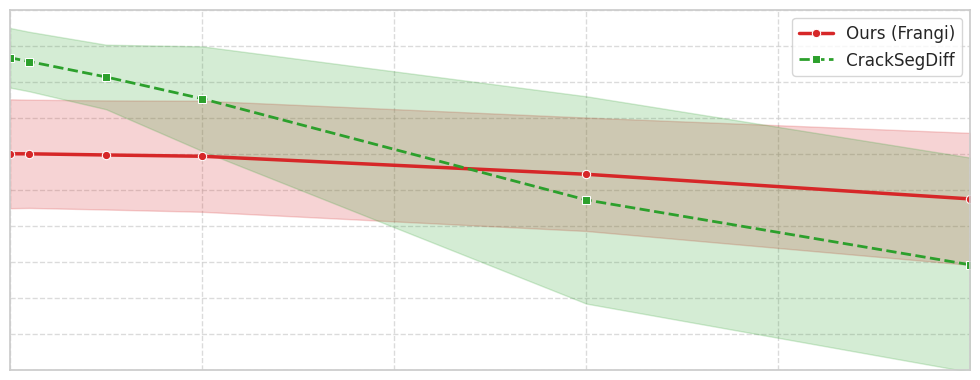
\includegraphics[width=.87\linewidth]{Jaccard_noisy.png}};
  \draw[-{Latex[length=1.6mm]}](plot.south west)--(plot.north west);
  \draw[-{Latex[length=1.6mm]}](plot.south west)--(plot.south east);
  \node[anchor=east,font=\scriptsize]at(plot.north west){100};
  \node[anchor=north east,font=\scriptsize]at(plot.south west){0};
  \node[anchor=north,font=\scriptsize]at(plot.south east){0.5};
  \node[anchor=south west,font=\small]at(plot.north west){Jaccard (\%) \citb{euvip26}};
  \node[anchor=north,font=\small,yshift=-3mm]at(plot.south){Noise level $s$};
 \end{tikzpicture}
 \par\vspace{1mm}
 
 {\scriptsize \textcolor{red}{\rule[.4ex]{7mm}{.7pt}} Our graph\quad
 \textcolor{green!50!black}{\rule[.4ex]{7mm}{.7pt}} CrackSegDiff \citb{cracksegdiff24}}
\end{column}
\begin{column}{.39\textwidth}
\vspace{-3mm}
\begin{gather*}
I_s=I(1+N), \qquad R_s=R+N'\\[.4mm]
N,N'\sim\mathcal N(0,s^2)\ \text{independent}
\end{gather*}
\vspace{-2mm}

\panel{.46}{IntensityNoisy_1FIND.png}{Noisy intensity}\hfill
\panel{.46}{ResultatNoisy_1FIND.png}{Our result, $s=0.5$}
\par\vspace{.5mm}
\begin{itemize}
 \item Slower degradation under added noise.
\end{itemize}
\end{column}
\end{columns}
\reffoot{euvip26,cracksegdiff24}
\end{frame}

\begin{frame}[t]{Transfer to geological images}
\vspace{-1mm}
\begin{columns}[T,onlytextwidth]
\begin{column}{.48\textwidth}
 \textbf{Vaches Noires} \citb{euvip26}
 \vspace{2mm}
 
 \panel{.475}{Test1_512_512_result.png}{Test 1\\\textcopyright\ Cerema}\hfill
 \panel{.475}{Test2_512_512_result.png}{Test 2\\\textcopyright\ Cerema}
 \vspace{2mm}
 
 {\scriptsize\textcolor{red}{Ours}\quad\textcolor{green!50!black}{Ground truth}\quad\textcolor{blue}{U-Net}}\par\vspace{1mm}
 \begin{itemize}
  \item IoU 47 / 50\% and 29 / 34\% (ours / adapted U-Net)
 \end{itemize}
\end{column}
\begin{column}{.48\textwidth}
 \textbf{Palais des Papes} \citb{euvip26}
 \vspace{2mm}
 
 \panel{.315}{PalaisDesPapes.png}{Intensity\\\textcopyright\ Cerema}\hfill
 \panel{.315}{PalaisDesPapes_IntDepth.png}{Depth overlay\\\textcopyright\ Cerema}\hfill
 \panel{.315}{PalaisDesPapes_Result.png}{Our result\\\textcopyright\ Cerema}
 \vspace{3mm}
 
 \begin{itemize}\setlength\itemsep{2mm}
  \item Main fracture recovered
  \item No retraining
 \end{itemize}
\end{column}
\end{columns}
\reffoot{euvip26}
\end{frame}

\divider{03}{Beyond pairwise connectivity}

\begin{frame}[t]{Toward order $K=2$}
\vspace{1mm}\centering
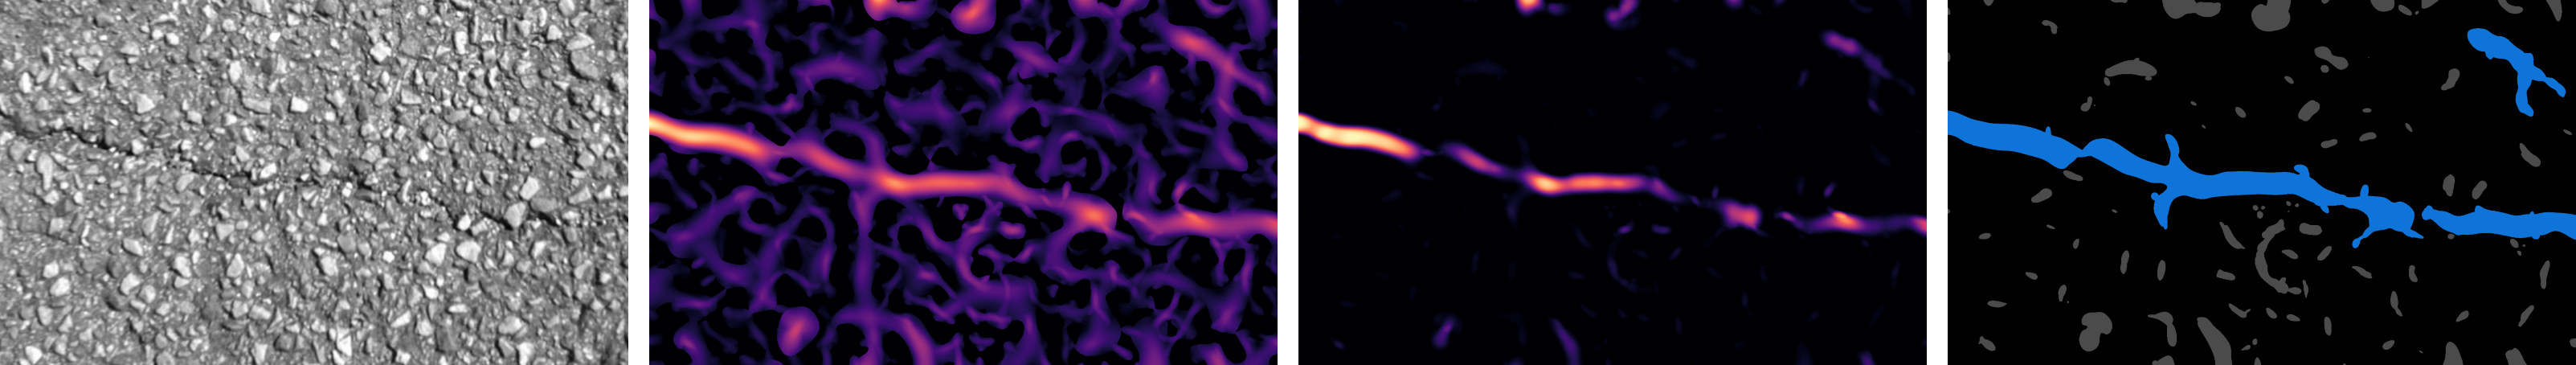
\includegraphics[width=.95\linewidth]{VTGraF_granularite.png}
\par\vspace{1mm}
\begin{minipage}{.95\linewidth}\scriptsize\centering
 \makebox[.245\linewidth]{granular image}\hfill
 \makebox[.245\linewidth]{pixel-wise \Frangi}\hfill
 \makebox[.245\linewidth]{graph similarity}\hfill
 \makebox[.245\linewidth]{retained component}\par
 \vspace{.7mm}VT-GraF \textcopyright\ Cerema
\end{minipage}
\vspace{2mm}

\begin{columns}[c,onlytextwidth]
\begin{column}{.46\textwidth}
\begin{itemize}\setlength\itemsep{3mm}
 \item Granular background can create spurious chains.
 \item $K=1$: connectivity through vertices.
 \item $K=2$: connectivity through triangles. \citb{ans26}
\end{itemize}
\end{column}
\begin{column}{.50\textwidth}\centering
\resizebox{\linewidth}{!}{%
\begin{tikzpicture}[x=1cm,y=1cm,every node/.style={font=\small}]
 \foreach \off/\k in {0/1,3.7/2}{\begin{scope}[xshift=\off cm]
  \coordinate(a)at(0,0);\coordinate(b)at(.65,.85);\coordinate(c)at(1.25,0);
  \coordinate(d)at(1.9,0);\coordinate(e)at(2.5,.85);\coordinate(f)at(3.1,0);
  \ifnum\k=1
   \draw[inria-rouge,line width=1.2pt](a)--(b)--(c)--(a) (c)--(d)--(e)--(f)--(d);
  \else
   \fill[inria-rouge!12](a)--(b)--(c)--cycle;
   \fill[inria-2024-bleu-canard!12](d)--(e)--(f)--cycle;
   \draw[inria-rouge,line width=1.2pt](a)--(b)--(c)--cycle;
   \draw[inria-2024-bleu-canard,line width=1.2pt](d)--(e)--(f)--cycle;
   \draw[gray,dashed,line width=.8pt](c)--(d);
  \fi
  \foreach \p in {a,b,c,d,e,f}{\fill[gris_fonce_inria](\p)circle(1.7pt);}
  \node[align=center]at(1.55,-.55){$K=\k$};
 \end{scope}}
\end{tikzpicture}}
\end{column}
\end{columns}
\reffoot{ans26}
\end{frame}

\begin{frame}[t]{Conclusion \& perspective}
\vspace{2mm}
\begin{columns}[T,onlytextwidth]
\begin{column}{.51\textwidth}
\textcolor{inria-2024-bleu-canard}{\textbf{Main steps}}
\begin{itemize}\setlength\itemsep{4mm}
 \item \Frangi{} filter $\rightarrow$ \Frangi{} graph \citb{euvip26}
 \item Multimodal fusion at the Hessian level
 \item Training-free extraction of crack skeletons
\end{itemize}
\end{column}
\begin{column}{.45\textwidth}
\textcolor{inria-rouge}{\textbf{Next steps}}
\begin{itemize}\setlength\itemsep{4mm}
 \item Evaluate higher-order connectivity
 \item Broader benchmarks
 \item Can a \Frangi{} graph hierarchy help guide SAM / CrackSAM?\par\citb{sam23}\ \citb{cracksam24}
\end{itemize}
\end{column}
\end{columns}
\vspace{2mm}
\centering
\resizebox{.48\linewidth}{!}{%
\begin{tikzpicture}[node distance=2mm,box/.style={draw=gris_fonce_inria!50,align=center,font=\scriptsize,text width=1.8cm,minimum height=8mm,inner sep=1pt}]
 \node[box,draw=inria-2024-bleu-canard,fill=inria-2024-bleu-canard!12,text=inria-2024-bleu-canard](g){\Frangi{}\\graph};
 \node[box,draw=inria-2024-bleu-canard,fill=inria-2024-bleu-canard!12,text=inria-2024-bleu-canard,right=of g](h){hierarchy};
 \node[box,draw=inria-rouge,fill=inria-rouge!12,text=inria-rouge,right=of h](s){foundation\\model};
 \draw[-{Latex[length=1.3mm]},inria-2024-bleu-canard](g)--(h);\draw[-{Latex[length=1.3mm]},inria-rouge](h)--(s);
\end{tikzpicture}}
\reffoot{euvip26,sam23,cracksam24}
\end{frame}

\begin{frame}[t,noframenumbering]{Bibliography: method and experiments}
\vspace{1mm}
\bibentry{frangi98}
\bibentry{gretsi25}
\bibentry{euvip26}
\bibentry{find22}
\bibentry{cracksegdiff24}
\end{frame}

\begin{frame}[t,noframenumbering]{Bibliography: higher order and perspectives}
\vspace{1mm}
\bibentry{ans26}
\bibentry{sam23}
\bibentry{cracksam24}
\end{frame}
\end{document}
